\externaldocument{Introduction.tex}
% \externaldocument{Experimental_Apparatus.tex}
\externaldocument{Results.tex}
\externaldocument{Analysis.tex}
\externaldocument{EIC_Jets.tex}
\externaldocument{Discussion.tex}
\chapter{Experimental Apparatus} 
A Large Ion Collider Experiment (ALICE) is the only experiment at the Large Hadron Collider (LHC) dedicated to studying heavy-ion physics. Its detectors measure and identify hadrons, electrons, photons, and muons. The ALICE detectors are optimized for the study of heavy-ion collisions up to the highest energy available and is designed to be simultaneously capable of measuring  bulk properties of the collision involving soft hadronic interactions and large cross section physics, and capable measuring rare probes involving small cross section physics. In particular, ALICE was designed to track and identify particles from very low,  \~100 MeV, up to $\approx$100 GeV, transverse momenta in an environment of extreme particle density. This chapter will first briefly discuss the LHC particle accelerator, followed by a description of the subdetectors and triggering system of ALICE.

\section{The Large Hadron Collider} 
\label{sec:LHC}

The LHC is the largest particle accelerator ever made. Located at CERN near Geneva, Switzerland, it was optimized to collide protons up to a center-of-mass energy of \sqrts=14 TeV, and heavy ions (including Pb, Ar, and Xe) up to \sqrtsNN=5.5 TeV \cite{Evans2008}.

The LHC was designed to supply a luminosity of $\mathcal{L}=10^{34}$cm$^-2$s$^-1$ for proton-proton collisions, and a luminosity of $\mathcal{L}=10^{34}$cm$^-2$s$^-1$. The proton-proton luminosity was driven by the search for the Higgs boson, with CMS and ATLAS considered as the high luminosity experiments at the LHC. The LHC was constructed using the existing tunnel of the Large Electron-Positron Collider (LEP), operational until 2000, and consists of 4 major components:

\begin{enumerate}
	\item Dipole magnets that bend the beam on its orbit with a maximum magnetic field of 8.33 T. 
	\item Quadrupole, sextupole, octupole and decapole magnets that focus the beams.
	\item Acceleration cavities that increase the beam energy.
	\item Two beam pipes with an ultra-high vacuum  which contain the two beams.
\end{enumerate}

The magnetic field in the dipoles is provided by superconducting magnets which are filled with liquid helium. The helium is cooled down to 1.9 K in order to reach the super-fluid state. To reduce the number of interactions of the beam with the environment or air, an ultra-high vacuum is kept in the beam pipes reaching a quality of $10^{-13}$ atm over a total volume of 150~m$^3$ \cite{Evans2008}.

The LHC has eight possible interactions points, four of them are equipped with large detector systems shown in Figure \ref{fig:lhc}. ALICE will be described in the next section. The detectors systems of ATLAS (A Toroidal LHC Apparatus) and CMS (Compact Muon Solenoid experiment) were designed as general purpose detectors primarily in pursuit of the Higgs-boson and its properties, as well as precision measurements of the Standard Model particles and searches for physics beyond the Standard Model. Although both detectors have not been optimized for heavy-ion collisions, they contribute extensively to the high \pt~analysis in Pb–Pb collisions, profiting from their large pseudorapidity coverage, excellent high luminosity capabilities, and high momentum resolution. The LHCb (LHC beauty) experiment dedicated its research program to the search for CP-violation in the B-meson system, as well as precision measurements in the charm and beauty quark sector.

\begin{figure}[htpb]
  \centering
	\includegraphics[width=0.6\textwidth]{Experimental_Aparatus/LHC.png}
	\label{fig:lhc}
	\caption{Overview of the CERN accelerator complex and the injection chains used for the LHC with their respective top energies for protons and ions after the respective accelerator \cite{zotero-342}.}
\end{figure}

\FloatBarrier

\section{A Large Ion Collider Experiment}
\label{sec:ALICE}
ALICE's aim is not to find signatures rare particles in pp collisions as is the primary focus of the other three major LHC experiments, but instead to collect as much data as possible from large heavy-ion events. This imposes strong demands on the detector. A Pb–Pb collision typically produces approximately 500-1000 charged particles per pseudo-rapidity unit, and can reach as high as $\text{d}N_{ch}/\text{d}\eta \approx 2000$ in the most central collisions \cite{ALICECollaboration2016}. Fig.~\ref{fig:alice} shows an overview of the ALICE detector.


\begin{figure}[htpb]
  \centering
  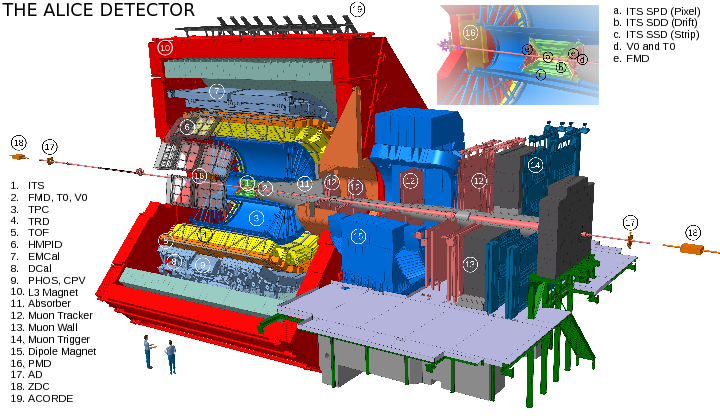
\includegraphics[width=0.99\textwidth]{Experimental_Aparatus/ALICE.png}
  \caption{Schematics of the ALICE detector \cite{Tauro2017}.}
  \label{fig:alice}
\end{figure}

As shown in Fig.~\ref{fig:alice}, ALICE can be conceptualized as consisting of three major parts:

\begin{enumerate}
    \item The central barrel contained inside the magnet with an acceptance in pseudo-rapidity of $-0.9 \leq \eta \leq 0.9$ over the full azimuth angle;
    \item The muon spectrometer at pseudo-rapidity of $-4.0 \leq \eta \leq -2.4$; 
    \item Various multiplicity detectors at $-3.4 \leq \eta \leq 5.1$
\end{enumerate}

The central barrel resides within the L3 magnet, a warm solenoid magnet with a magnetic field of B = 0.5 T. The muon spectrometer extends only in the forward region (C side) and contains a dipole magnet (B = 0.67 T) which bends the muons away from the interaction vertex in the horizontal plane. Lastly, the multiplicity detectors are arrays of scintillator counters, with one in each of the forward regions.

\subsection{Inner Tracking System}
\label{sec:ITS}
Closest to the interaction point, in the middle of the central barrel, is the Inner Tracking System (ITS) covering the pseudorapidity window $|\eta| < 0.9$. The ITS is used for triggering and high-resolution tracking and consists of six concentric layers of silicon detectors surrounding the beam pipe: two layers each of Silicon Pixel Detectors (SPD), Silicon Drift Detectors (SDD), and Silicon Strip Detectors (SSD). 

A schematic overview of the ITS is given in Fig.~\ref{fig:ITS}. The main purposes of the ITS are to accurately measure the position of the collision vertex and secondary vertices from weakly decaying particles (in particular strange hadrons and B and D mesons, which have typical decay lengths of a couple of cm), measure the \pt~and position of charged particle tracks -- often complementing TPC tracking information -- and, in the case of the SPD, to provide triggering input for the entire detector. 

This detector system has a very fine granularity, resulting in a high tracking and vertexing resolution even in extremely high multiplicity environments. The resolution for each subsystem is summarised in Table~\ref{tab:its}. 

\begin{figure}[htpb]
  \centering
  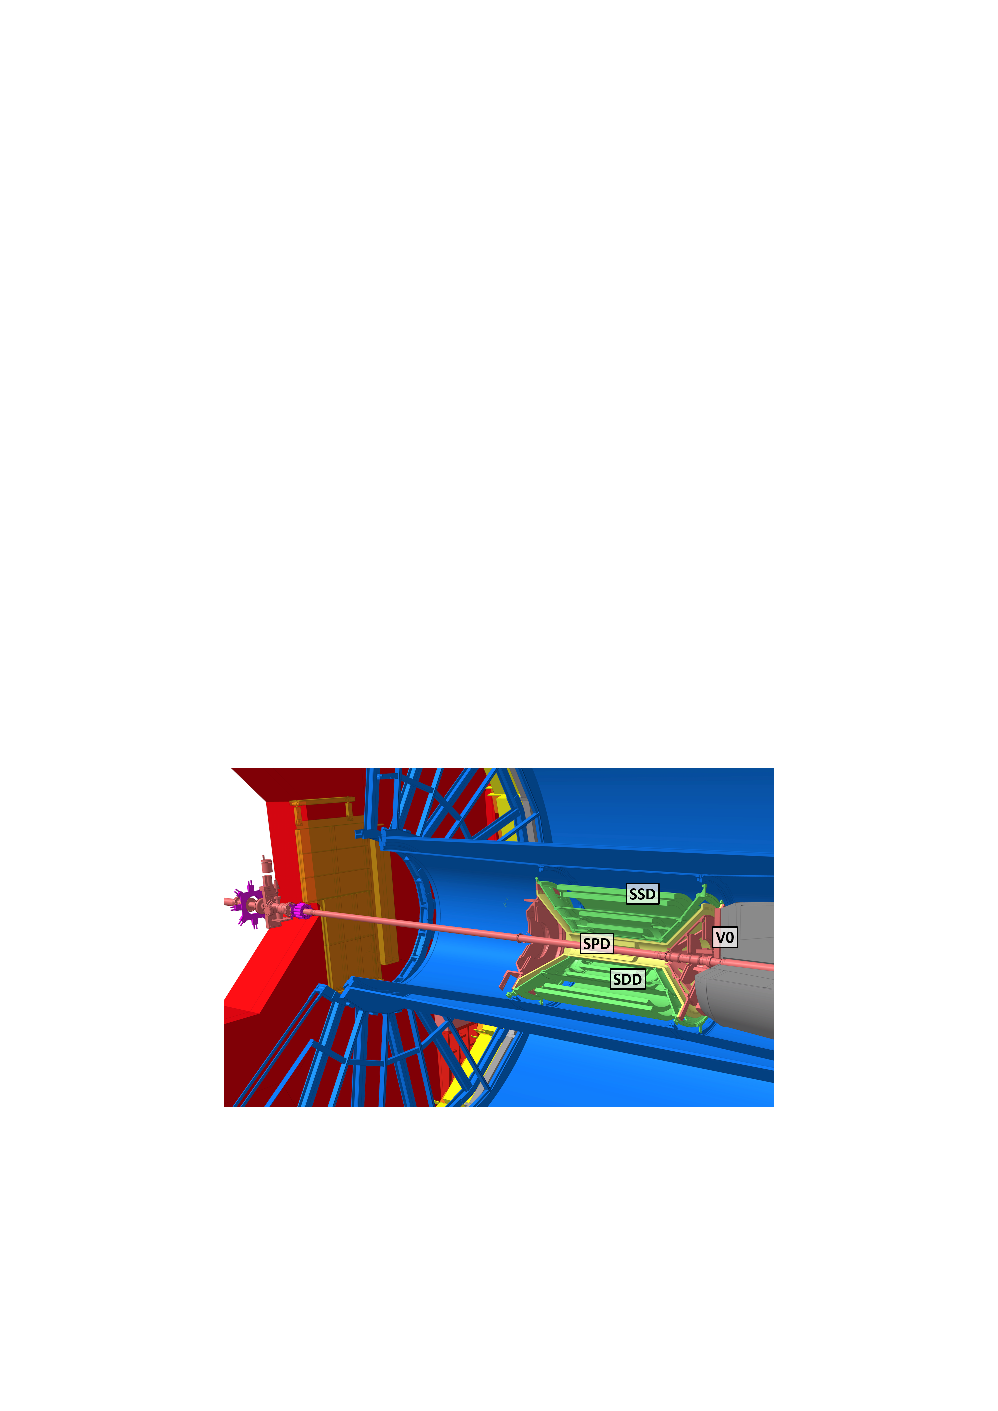
\includegraphics[width=0.8\textwidth]{Experimental_Aparatus/ITS.pdf}
  \caption{Schematics of the Inner Tracking System and nearby detector components, modified from \cite{Tauro2017}. The V0 detector is only shown on the C side.}
  \label{fig:ITS}
\end{figure}

\begin{table}
\centering
\begin{tabular}{ c c c }
        \hline
	Detector & $r\varphi$ precision ($\mu$m) & $z$ precision ($\mu$m)\\
	\hline
	SPD & 12 & 100 \\
	SDD & 35 & 25 \\
	SSD & 20 & 830 \\
	\hline
\end{tabular}
  \caption{Coordinate resolution in azimuthal $r\varphi$ and longitudinal ($z$) directions for each subsystem in the ITS \cite{Contin_2012}.}
  \label{tab:its}
\end{table}


The ITS is a silicon based detector. Silicon is a semiconductor meaning it has a valence band and a conduction band separated by a band gap. The basic operating principle is as follows: a pn junction is used where a reverse bias is applied that depletes the active area of charge carriers. When a charged particle hits the detector, it will create electron-hole pairs along its trajectory that will in turn generate a current pulse, as shown in Fig.~\ref{fig:silicon}. The current will then traverse the electric field and eventually be collected at electrodes connected to a current amplifier. For the purposes of charged particle tracking with the ITS, the only relevant information is whether a particle has hit the detector. This is ensured by reading out only if the pulse is above a certain threshold. The advantages of using a semiconductor are that this creates a fast signal, and one can achieve a very high tracking resolution while maintaining a low material thickness, since the electron diffusion length is only a few $\mu$m. The material thicknesses of each ITS layer ranges from 0.83 to 1.26 $X/X_0$\% \cite{Contin_2012}, with the SPD layers being the thinnest, and one of the SDD layers being the thickest.

\begin{figure}[htpb]
  \centering
  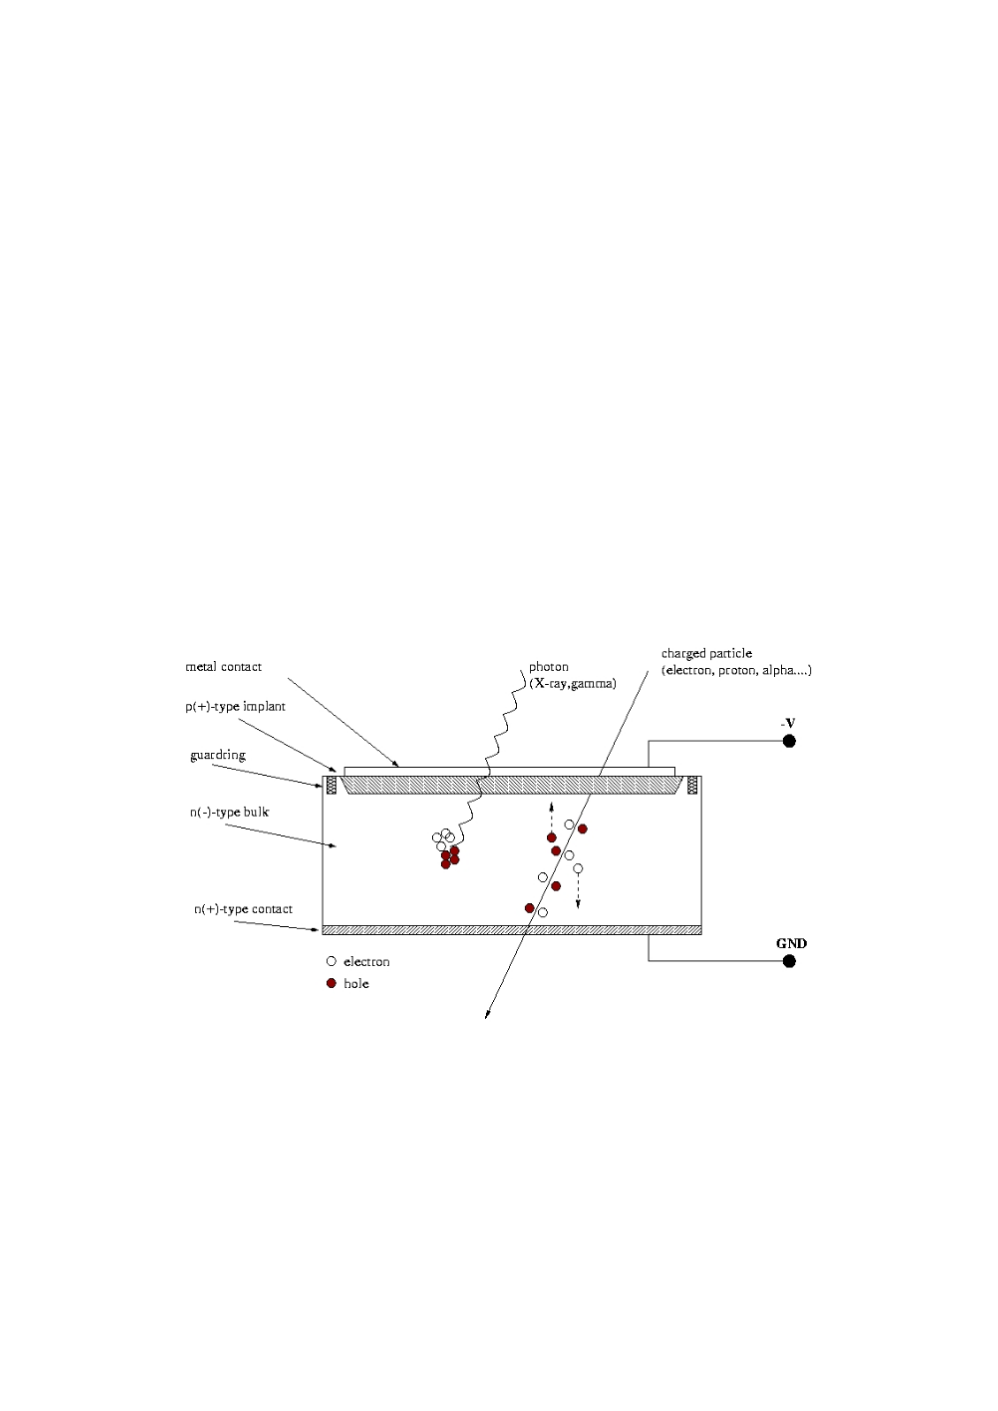
\includegraphics[width=0.8\textwidth]{Experimental_Aparatus/silicon_detector.pdf}
  \caption{Basic principle of a semiconductor detector. When a charged particle traverses the detector, it excites electrons from the valence band to the conduction band, which creates electron-hole pairs. The applied electric field will cause these to drift towards the metal contacts, which generates a current pulse that can be detected \cite{Brenner}.}
  \label{fig:silicon}
\end{figure}

Each subdetector of the ITS uses a different technology. The SPD is built of pixels of silicon diodes, each measuring 50×425 $\mu$m$^2$. These are read out by 1200 chips per layer, each covering 8192 cells, totalling 9.8$\times$106 cells per layer. The two SPD layers are located 3.9 and 7.6 cm from the beam axis, respectively, and extend 282 mm in the longitudinal direction.

The SDDs are built of 260 drift cells distributed over the two layers, where the drift time of charge carriers is measured in order to precisely determine where the track has interacted with the cell. Each cell has 256 collection anodes mounted to it along the z axis with a spacing of 294 $\mu$m. The drift regions are 35mm long and extend in the $\varphi$ direction. To determine the $r\varphi$ coordinate, the drift velocity is monitored by MOS injectors in the substrate that are triggered during gaps in the LHC bunch crossing schedule so they do not interfere with collisions. The position is determined by integrating the velocity over the time measured at the anode. The effective cell length is $\leq 202\mu$m. These detectors are able to measure the number of collected charge carriers, which is proportional to the energy deposited per unit length, dE/dx, and therefore can be used for PID. The two SDD layers are located 15.0 and 23.9 cm from the beam axis and have lengths of 443 and 593 mm in the z direction.

Finally, the SSDs each consist of a double layer of silicon strips placed at an angle of 35 mrad ($\approx 2\textdegree$) relative to each other. When a particle crossing one of the SSDs yields a signal in both strip layers, the result will be a detection at the crossing point. The number of collected charge carriers is measured, again providing $dE/dx$ information in the SSD. The strips have a width of 95 $\mu$m. However, due to the arrangement of the strips, the effective resolution is better than what the width alone might predict in $r\varphi$, but worse in z. In total, 1.15$\times$106 strips are used in the inner layer and 1.46$\times$106 strips in the outer layer. The inner and outer SSD layers are located at 38 and 43 cm from the beam axis, respectively, and extend 86 and 98 cm in the z direction.


\subsection{V0 Detector}
The V0 detector is made up of two circular arrays of scintillator counters, with one at each of the forward regions of the ALICE detector. The array on the A side (V0A; opposite to the muon arm) is placed 300 cm from the collision vertex and covers the pseudorapidity region $2.8 < \eta < 5.1$. In order to accommodate the muon absorber, however, the V0C array is instead placed only 90 cm from the vertex, covering $-3.7 < \eta < -1.7$ (this is why V0C is visible in Fig. 4.2, but not V0A). Each array consists of 4 layers with 8 scintillators each, each covering a circular segment spanning 45 $\textdegree$ in azimuth. The resulting granularity is, while not fantastic, is sufficient for the main purpose of the v0 detector: Triggering and multiplicity measurements.

\subsection{Time Projection Chamber}
\label{sec:TPC}

The Time Projection Chamber (TPC) is the largest tracking detector in ALICE. It as a gaseous detector that relies on the ionization of a gas for the detection of charged particles. A charged particles travels the gas, they create a trail of ionization. The electric field applied through the volume of the TPC causes the electrons (ions) to drift towards the anode (cathode). In the ALICE TPC, thin wires with an applied voltage serve as anodes, resulting in a very strong magnetic field near the anode, which drops off as the distance from the anode increases. Electrons sufficiently accelerated in this field will give rise to secondary ionizations and a subsequent chain reaction known as avalanche multiplication. The detector system can then detect these induced voltage pulses at the cathode readout plane, but the voltage pulse will not stop until the ions with a much slower drift velocity than electrons are collected at the cathode, making the detector relatively slow. This process is illustrated in Fig.~\ref{fig:tpc_avalanche}.

\begin{figure}[htpb]
  \centering
  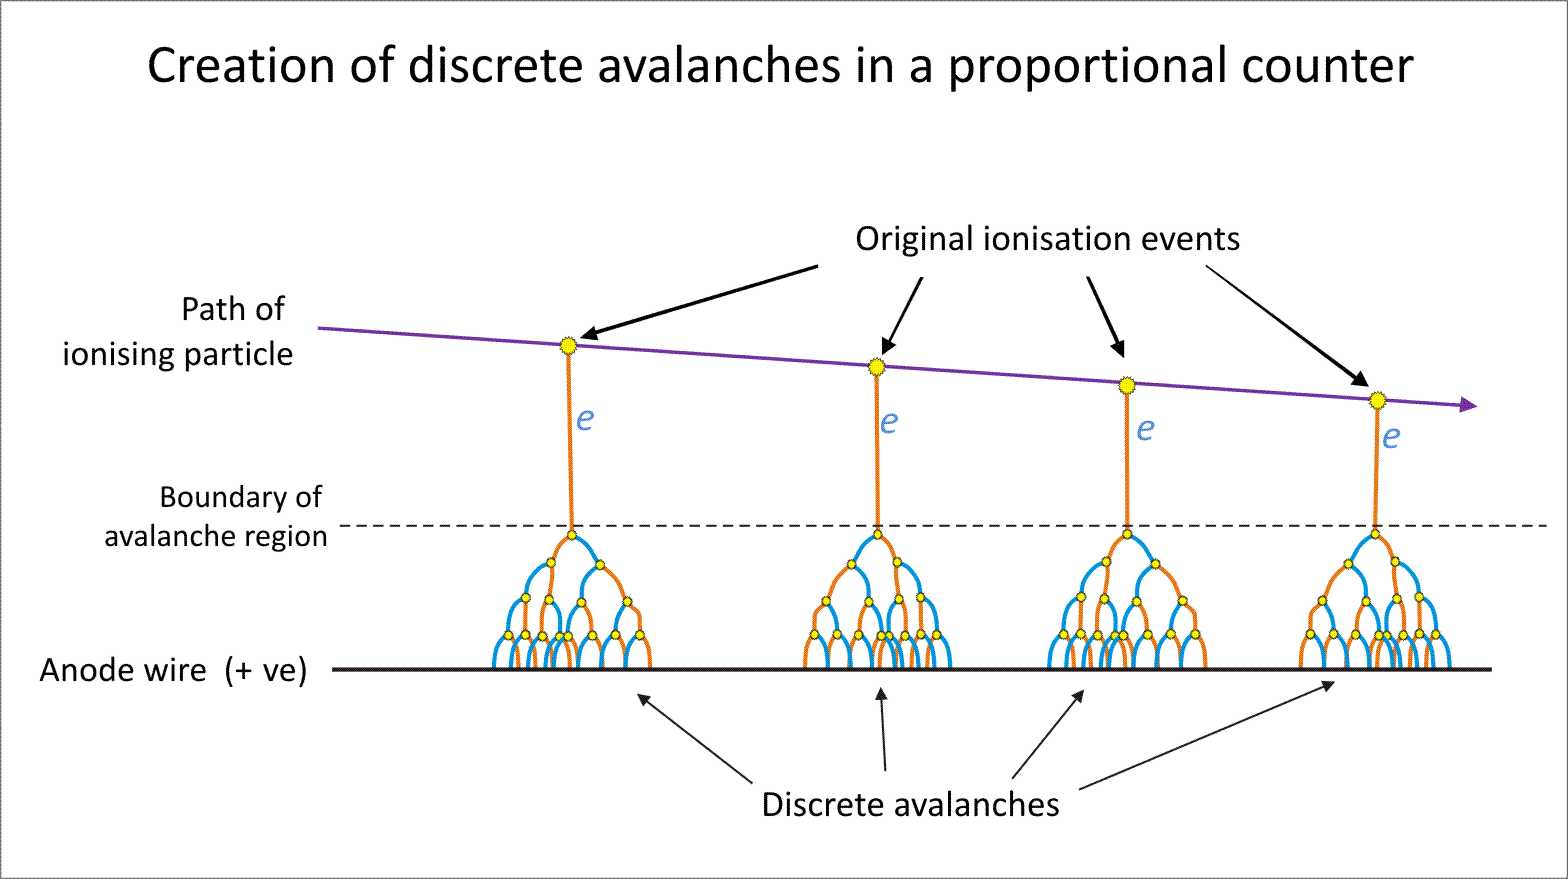
\includegraphics[width=0.8\textwidth]{Experimental_Aparatus/Proportional_counter.jpg}
  \caption{Principle of avalanche multiplication in a gas detector \cite{Dougsim2012}.}
  \label{fig:tpc_avalanche}
\end{figure}

If there is insufficient voltage to cause such an avalanche, the energy deposited at the electrodes is proportional to the number of initial ionisations alone, and this is proportional to the energy deposited per unit length, $\text{d}E/\text{d}x$. This provides PID information. Consequently, the voltage of the anodes are lowered and placed such that they can be in state called ``proportional mode''.

The ALICE TPC has a cylindrical geometry surrounding the ITS. It has an inner radius of 85 cm, an outer radius of 250 cm, and an overall length of 500 cm. A longitudinal electric field is applied over the cylinder, divided in the center by a cathode plate.  A voltage of 100 kV is applied between the center and endcaps; the resulting field strength within the detector volume is 400 V/cm. At the endcaps are Multi-Wire Proportional Chambers (MWPCs), arrays of anode wires operating in proportional mode. When a charged particle from the collision traverses the gas, electron-ion pairs will be created along its trajectory. Idealy, the field is longitudinal with minimal space charge distortions such that the electrons will be projected onto the endcaps, giving precise information about the (r, $\varphi$) coordinates of the trajectory. The drift velocity is carefully monitored using a laser system, which also detects inhomogeneities in the electric field. The laser system produces planes of tracks in the detector perpendicular to the electric field that make it easy to measure drift time as well as deviations caused by distortions. With a well determined drift velocity, the z coordinate is obtained by measuring the arrival time of the electrons. For the most frequently used TPC gas mixture – 85.7\% Ne, 9.5\% CO$_2$, and 4.8\% N$_2$ – this results in an average drift velocity of 2.65 cm/$\mu$s for the electrons, or an overall drift time of 94 $\mu$s for the longest drift distances. The endcaps are divided into 18 sectors, with four readout chambers each – two inner readout chambers (IROCs) and two outer readout chambers (OROCs). The wire density is higher for the IROCs as they are closer to the beam pipe, and the voltage applied is slightly lower. There are no anode wires between the sectors, resulting in gaps in the detector acceptance. The readout chambers have three layers of wires. The innermost wires are thin anode wires spaced 2.5 mm from each other. The middle layer consists of thicker cathode wires, where the ions released during avalanches are collected. The signal is read out from cathode pad planes, with a size in ($r,r\varphi$) space ranging from 4$\times$7.5 mm$^2$ in the IROCs to 6$\times$15 mm$^2$ in the outermost OROC sector. This results in a total number of 159 radial clusters \cite{Alme2010}.


The operation of the TPC is usually a delicate balance. If the voltage is too high in the normal operational mode, photons released in the de-excitation of gas ions may trigger additional avalanches that skew the initial signal. Another issue has to do with the recombination of ions and electrons at the electrodes, where gas atoms may again enter an excited and prolong the avalanche. To prevent this, a molecular component – usually CO$_2$ or an organic molecule – is added as a quencher to the gas. Unfortunately, at the high interaction rates delivered in Run 2, unexpectedly large space-charge distortions were observed at very specific regions of the TPC. They appeared at the boundaries between certain IROCs and deflect the ionization electrons towards these boundaries, leading to a bias in the measured space-point position and effectively decreasing the active readout area. It was suspected that insufficient insulation of some wires in this area could cause strong electric fields leading to amplification and therefore columns of ions drifting back from in between the readout chambers. After the TPC was brought to the surface at the beginning of LS2 indeed tips of anode wires sticking out of the ledges were found on all affected chambers near the expected radii~\cite{Schmidt2020}. A reduction of the distortions in the hot spots by a factor of about 4 was achieved with the special voltage settings in 2018 compared to 2015~. These space charge distortions are shown in Fig.~\ref{fig:tpc_distortion}.

\begin{figure}[htpb]
  \centering
  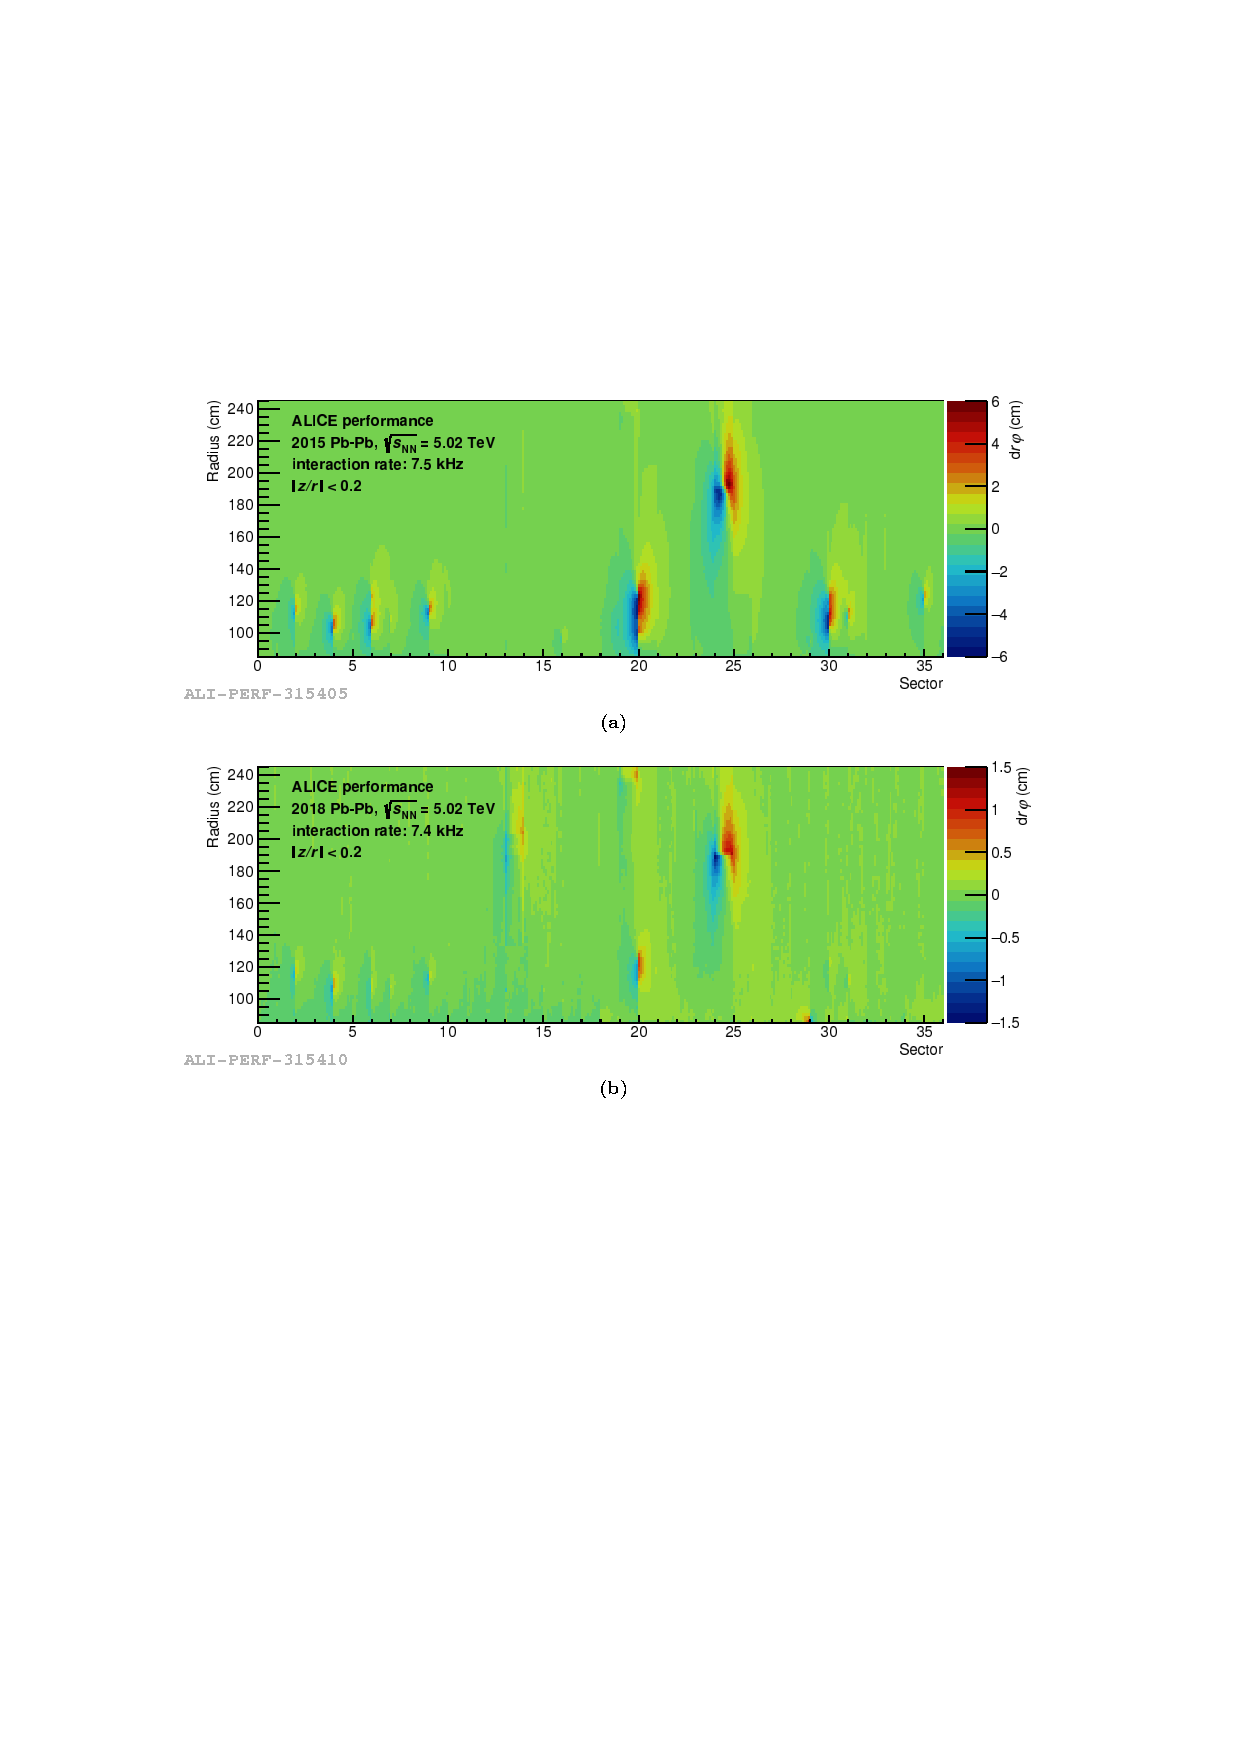
\includegraphics[width=0.8\textwidth]{Experimental_Aparatus/TPC_distortion.pdf}
  \caption{Measured space-charge distortions in $r\varphi$ near the central electrode are shown for Pb–Pb runs with high interaction rates in 2015 (upper plot) and 2018 (lower plot). For both runs the TPC was filled with argon. Note the different z-axis scales. \cite{Hellbar2019}}
  \label{fig:tpc_distortion}
\end{figure}


For the pp and \pPb~data used in this analysis, the TPC was not read out or was compromised for several runs. In order to maximize the statistics for the pp and \pPb, ITS-only tracking was used, a first in ALICE for two-particle correlations. The performance of ITS-only tracking vs. the standard TPC+ITS tracking is discussed in detail in Sec.~\ref{sec:tracking_published_comparision}.

\FloatBarrier
\subsection{Electromagnetic Calorimeter}
\label{sec:EMCal}

The Electromagnetic Calorimeter (EMCal) and Di-Jet Calorimeter (DCal) were mainly designed to measure high \pt~objects. Originally, the calorimeter system in ALICE was a layered lead-scintillator sampling calorimeter attached to wavelength shifting fibers for light collection \cite{Blau2020}, covering $107\textdegree$ in azimuth and  $|\eta| < 0.7$ in pseudorapidity. However, in order to enable the study of di-jet-events using full jets (rather than jets reconstructed with charged particle tracking alone), the calorimeter system was extended in 2010 to also include the DCal. The DCal is approximately opposite in $\varphi$ and uses the same design as the EMCal. The EMCal ond DCal are made up of 12288 and 5377 towers (also called cells), respectively. Each tower has a cross-sectional area approximately twice the Moli'ere radius of $\Delta\eta\times\Delta\varphi = 0.0143\times0.0143$ with a depth of 24.6 cm that corresponds to approximately 20 radiation lengths. The calorimeters are organized into modules comprised of $2\times2$ cells. These modules are further organized into 10 supermodules that are made up of up to $12\times24$ modules in the EMCal. Fig.~\ref{fig:emcal} (left) shows the EMCal made up of these supermodules, while (right) shows the various components that make up a single module.

\begin{figure}[htpb]
  \centering
  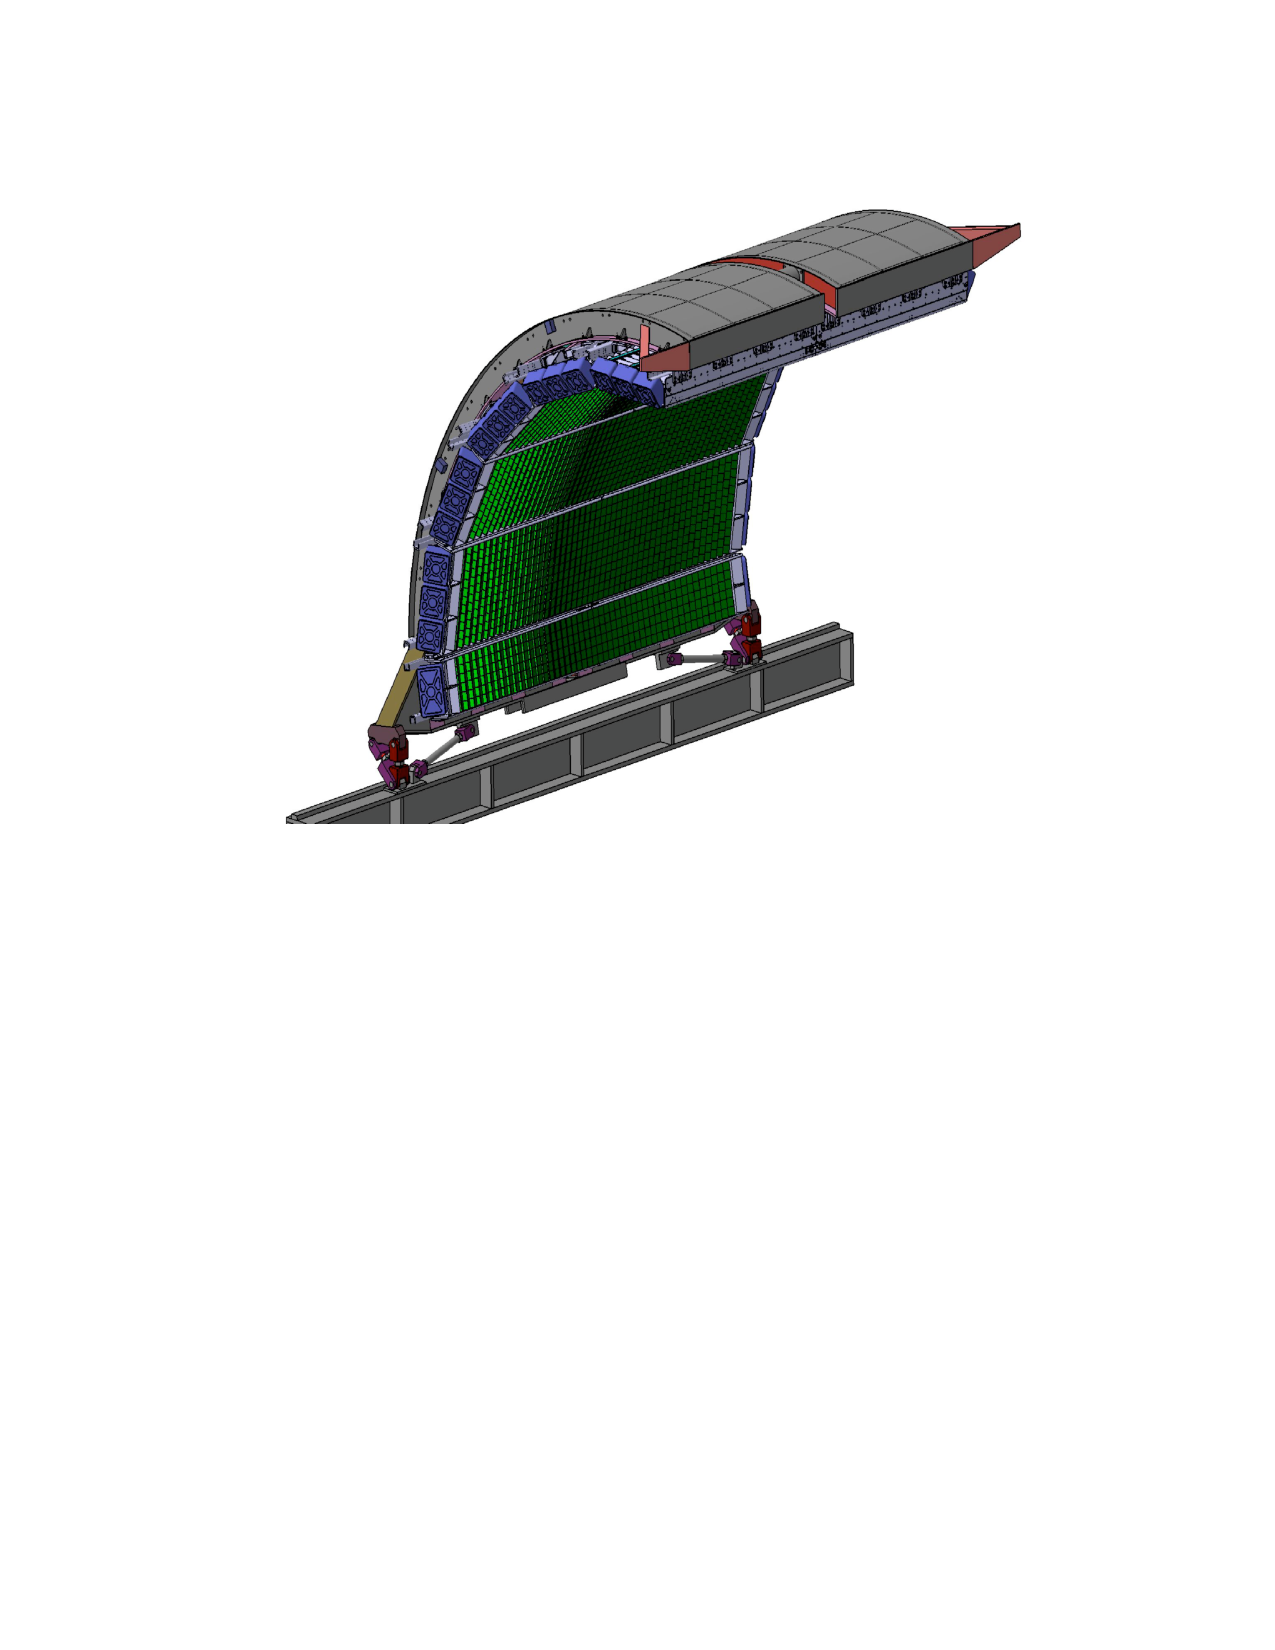
\includegraphics[width=0.45\textwidth]{Experimental_Aparatus/emcal.pdf}
  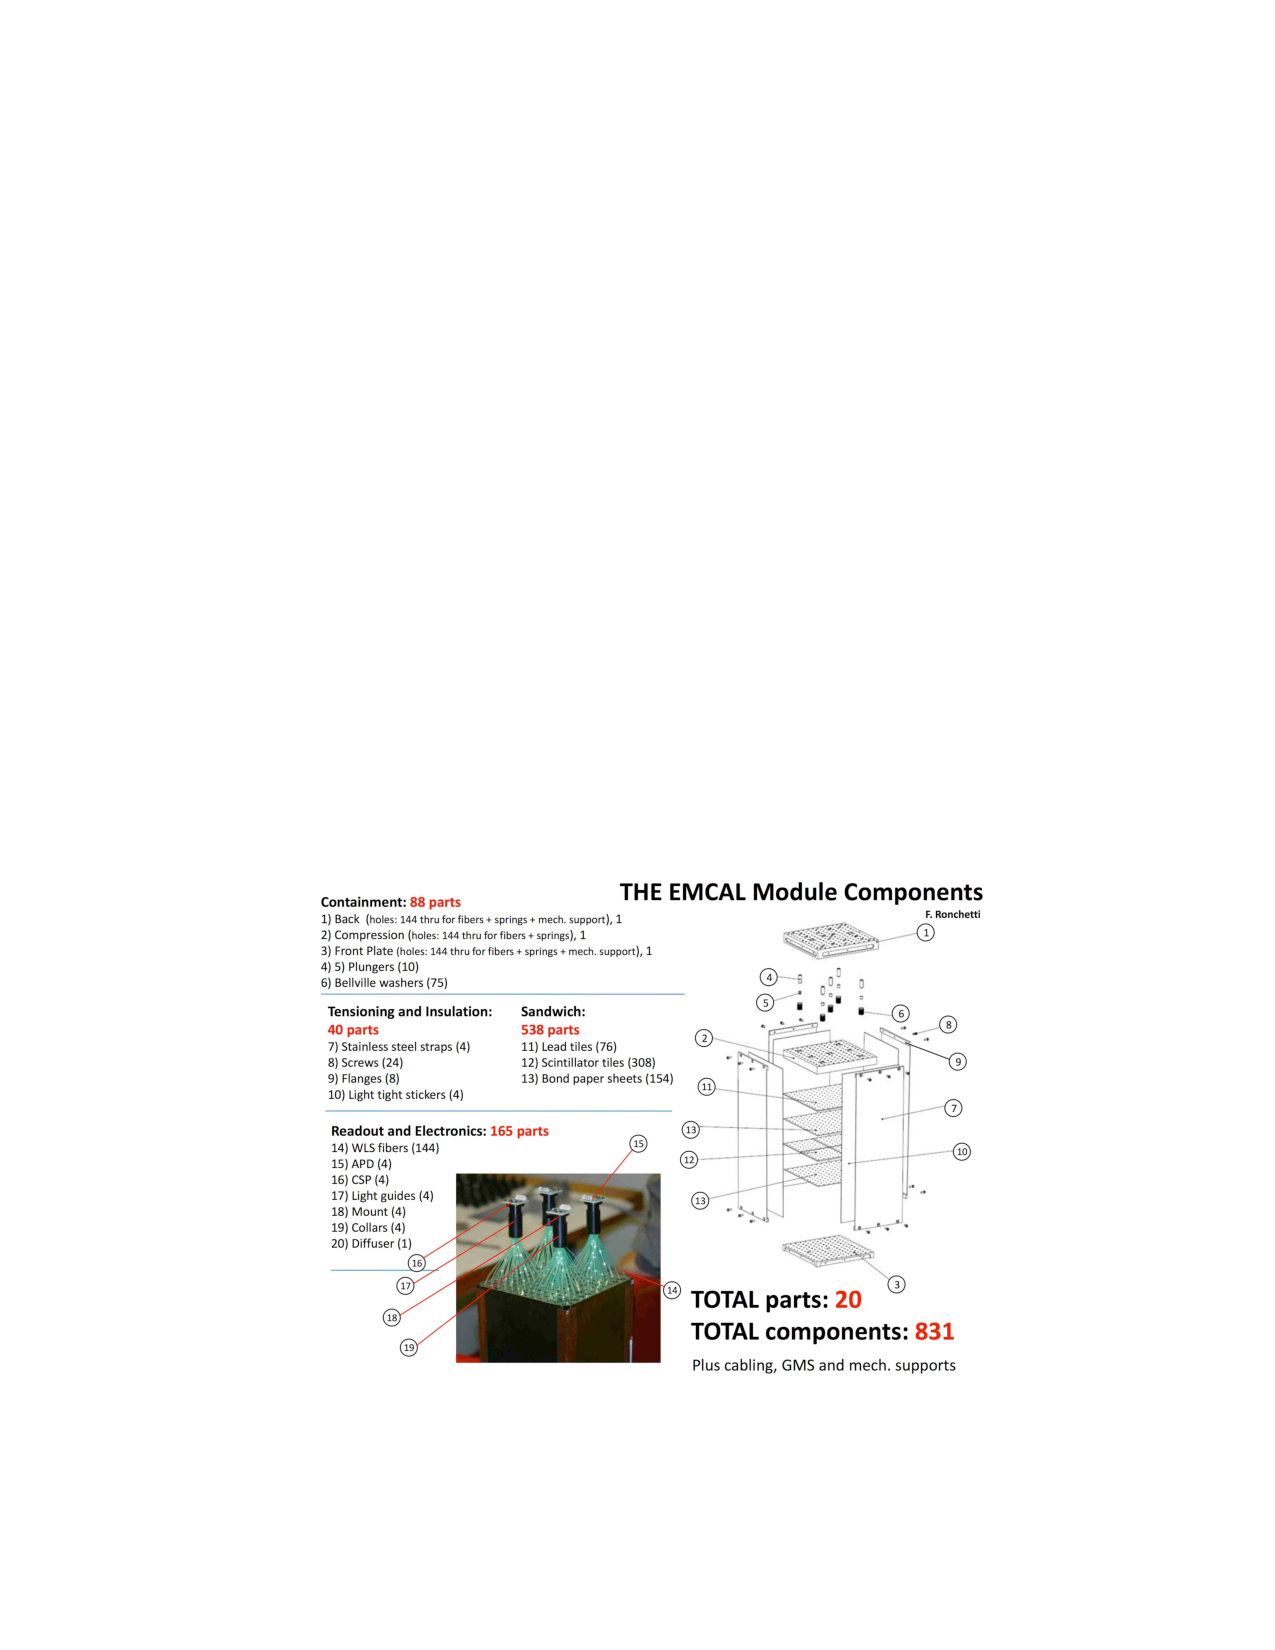
\includegraphics[width=0.45\textwidth]{Experimental_Aparatus/module.pdf}
  \caption{Left: The array of Super Modules shown in their installed positions on the support structure. Right: Exploded view drawing of EMCal module showing all components. Adapted from \cite{Bellwied2010}.}
  \label{fig:emcal}
\end{figure}


The wavelength shifting fibers are wired such that the scintillation light from each cell is read out by a $5\times5$ mm$^2$ avalanche photodiode. The relative energy resolution of the calorimeter is $\sigma/E = 1.7\% \oplus 11.3\%/\sqrt{E} \oplus 4.8\%/E$ for the energy range of interest for this analysis (roughly 10-50 \GeVc).


\subsection{Time of Flight Detector}
\label{sec:TOF}
The working principle of the TOF detector is to measure the time-of-flight from the interaction point of a particle in order to determine its velocity. Combined with the momentum information, one can extract the mass of the particle. The arrival time measurement is achieved by an array of Multi-gap Resistive-Plate Chambers (MRPCs). MRPCs are thin gaseous detector cells that have a high and uniform voltage of 6500V applied to them~\cite{Carnesecchi2019a,Aamodt:2008zz}. These are divided into two half-cells, each further divided into five smaller modules blocked by resistive glass plates. The field is sufficiently strong enough such that avalanche multiplication can occur, and thus a particle traversing the cell gives rise to a detectable signal. The glass plates block the avalanches, in order to reduce the time jitter, which scales with the propagation distance. The signals from each gap sum up to the total signal, and using multiple gaps increases the signal strength. The achieved time resolution is about 40 ps.

\begin{figure}[htpb]
  \centering
  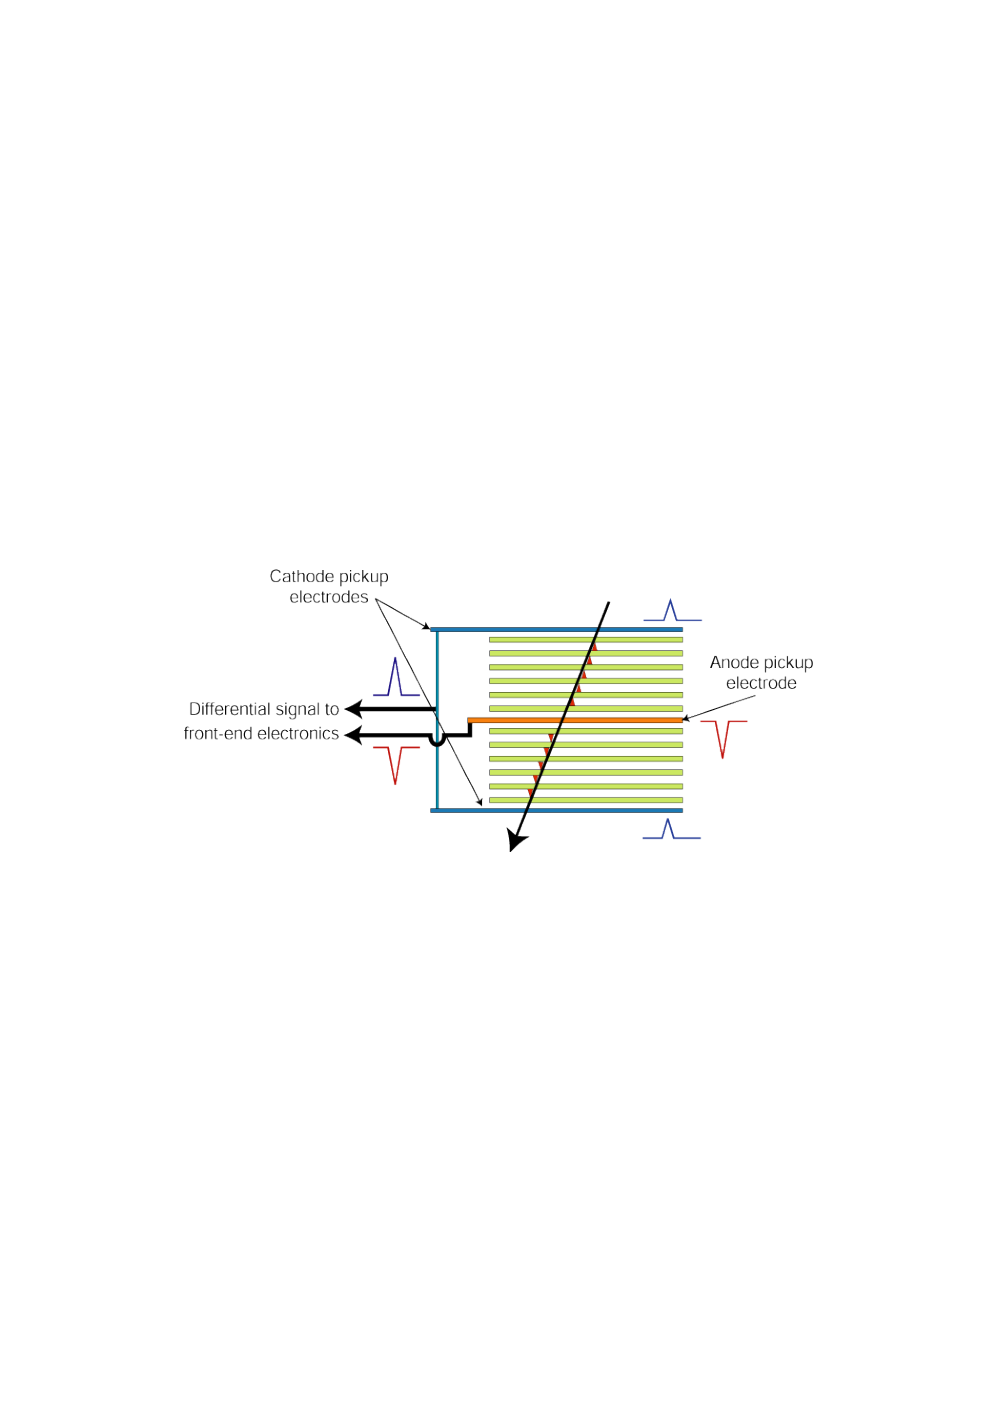
\includegraphics[width=0.8\textwidth]{Experimental_Aparatus/TOF.pdf}
  \caption{Working principle of a TOF detector cell. A charged particle entering the cell will give rise to avalanches in the gas, which are blocked by glass plates mounted inside the cell. The resulting electrons will be picked up at the anode, which divides the cell into two half cells. Adapted from \cite{Adolfsson2020}.}
  \label{fig:TOF}
\end{figure}

The TOF detector has full azimuthal coverage and covers the pseudorapidity region of $|\eta| < 0.9$. The inner radius of the TOF is 370 cm with an active length of 741 cm. A total of 157,000 cells are arranged into 122$\times$13 cm$^2$ strips and put in 18$\times$5 modules (in ($\varphi,z$) space). The strips overlap each other to achieve full coverage within each module. In order to minimize the path length of particles coming from the collision, the modules are tilted so that each strip is facing the interaction point perpendicularly.

\section{Central Barrel Tracking}

A tracking algorithm must be used in order to reconstruct the particle tracks from hits in the detector. ALICE uses a Kalman filter algorithm. A Kalman filter uses a parametrisation of the track and optimises trajectories through the addition of additional space points. The algorithm is initiated with a seed, usually consisting of a few clusters in the outer layers of the TPC (the exception of course being the use of ITS-only tracking). An initial approximation of the track is made with the assumption that the track originates from the collision vertex, and is further extrapolated from hits in the SPD. The process is repeated by removing this constraint to account for the possibility that the track actually originates from a secondary vertex. The track information is continually improved by propagating the track \textit{inwards} and adding additional space points within 4 standard deviations of the best guess of the trajectory while accounting for multiple scattering and energy loss inside detector material. After each iteration, the parameters of the trajectory as well as the covariance matrix of the parametrisation are updated to improve accuracy. If more than one detector hit satisfies the selection criteria, multiple different propagations are tested, and the tracks with the lowest $\chi^2$ are selected at the end.

As the track is propagated from the outer edge of the TPC inwards, the tracking is further improved by adding hits from the ITS once the inner edge of the TPC is reached. For tracks where the primary vertex constraint has been lifted within the TPC, the same constraint is initially applied to ITS tracks, but repeated without the constraint as well: the higher precision of the ITS makes it possible to find secondary vertices that are much closer to the primary vertex. For tracks where the primary vertex constraint has already been lifted in the TPC, the ITS tracking is done once without imposing the constraint.

Once the track propagation is completed in both the TPC and the ITS, the Kalman filter algorithm is reversed by using track parameters from the first procedure as an initial guess, but this time starts from the innermost layer of the ITS and propagates \textit{outwards}. The second iteration is applied in order to remove outliers from the initial track propagation. Once this iteration reaches the outer edge of the TPC, there is an option to incorporate hits from the other detector subsystems such as the Transition Radiation Detector (TRD), and eventually the TOF (as well as others), but this option is not used in this analysis. The main analysis of this thesis uses ITS-only tracking due to the space charge distortions of the time projection chamber discussed in Sec.~\ref{sec:TPC}. This results in tracks with fewer space points as input to the Kalman filter track reconstruction, but the performance was found to be comparable to the traditional ITS+TPC Hybrid tracking low multiplicity pp and \pPb, Sec.~\ref{sec:tracking_published_comparision}.

\section{Triggering System}
\label{sec:trigger}


ALICE is capable of operating at an event rate of a few kHz. The LHC bunch crossing rate, however, is 40 MHz. Even though not all bunch crossings result in a collision, an extensive triggering system is required to reduce the event rate and ensure all particles detected in an event are in fact from the same collision. This is needed despite the that fact that during pp collisions, the accelerator is actually tuned such that the luminosity at ALICE is $\mathcal{L}\approx 10^{30}-10^{31}\text{cm}^{-2}\text{s}^{-1}$, much lower than at ATLAS or CMS with a luminosity of $\mathcal{L}\approx 10^{30}-10^{31} \text{cm}^{-2}\text{s}^{-1}$. This reduces pile-up, but also the effective collision rate \cite{Wenninger:2668326}.

 The V0 and SPD detectors are the most important detector subsystems for triggering. The trigger input is handled by the Central Trigger Processor (CTP) that sends a command to all active detectors once it receives a successful trigger. There are three levels of triggers: L0, L1, and L2, and events are only accepted if the highest level, L2, triggers successively. The L0 trigger is simply synchronised with the LHC bunch crossing clock and includes the fastest inputs processed within 1.2 $\mu$s after the collision. Additional inputs that take longer than 1.2 $\mu$s and up to 6.5 $\mu$s are handled by the L1 trigger. The L2 trigger then handles all the slower inputs, with the restriction that it must be completed before the TPC needs to be read out, less than $88 \mu$s after the collision. 

The signals used by the trigger depend on the trigger configuration. One important configuration is minimum bias (MB), that selects against non-collisions. The MB trigger requires a hit in the both the V0A and V0C detectors. In order to reduce beam-gas events, additional requirements on the V0 timing information and on the correlation between the number of tracklets and clusters in the SPD are enforced. MB events are used in this analysis in the event mixing as well as in the ITS only tracking validation. Another trigger configuration is EG1, as well as EG2. These triggers require a hit in the EMCal up to a certain threshold before tracks can be read out for the event. For EG1, this threshold is 11 \GeVc, and 5 \GeVc~for EG2. 

Once the CTP receives a successful trigger, the CTP will begin a series of read-out operations for each active detector until eventually the trigger input is recorded locally at a Local Data Concentrator (LDC). During this processing, the read-out system will of course be busy, and a signal will be sent to the CTP that blocks triggering until the detectors are ready again. Some of the data from this read-out process are duplicated and sent to the High Level Trigger, where it is processed and decided whether the event should be stored permanently or rejected. This is the final triggering stage. If accepted, the data are compressed by rejecting irrelevant information and the remaining event data sent to Global Data Concentrators (GDCs) through the Data Acquisition (DAQ) system. The whole event is built from detector readouts in the GDCs, and is stored in first in Transient Data Storage. Some of the data is also processed online through data quality monitoring and detector algorithms to further reject bad quality events. For run two, the data quality monitoring is manual, and if there is a deterioration in quality, the shift leader may decide to stop a run until the problem is resolved. After all checks are passed, the data, several TB to PB, will be sent to the GRID for final storage, post-processing, and to be copied to tape.


% Because the data is so large and often inconvenient to pull for a single analysis, batches of analyses that need access to same dataset are grouped together in \textit{trains}. A train is then sent to the GRID to process a specific set of runs, and is the nominal way most analysis in ALICE are done. %often with at least one to two days between analysis iterations. The Berkeley group, however, takes a different approach to this method, discussed in more detail in \ref{sec:ntuples}.


